% Compile: pdflatex -interaction=nonstopmode -halt-on-error fig_certicut_architecture.tex
\documentclass[tikz,border=6pt]{standalone}
\usepackage{amsmath,amssymb}
\usetikzlibrary{arrows.meta,positioning,calc}

\begin{document}
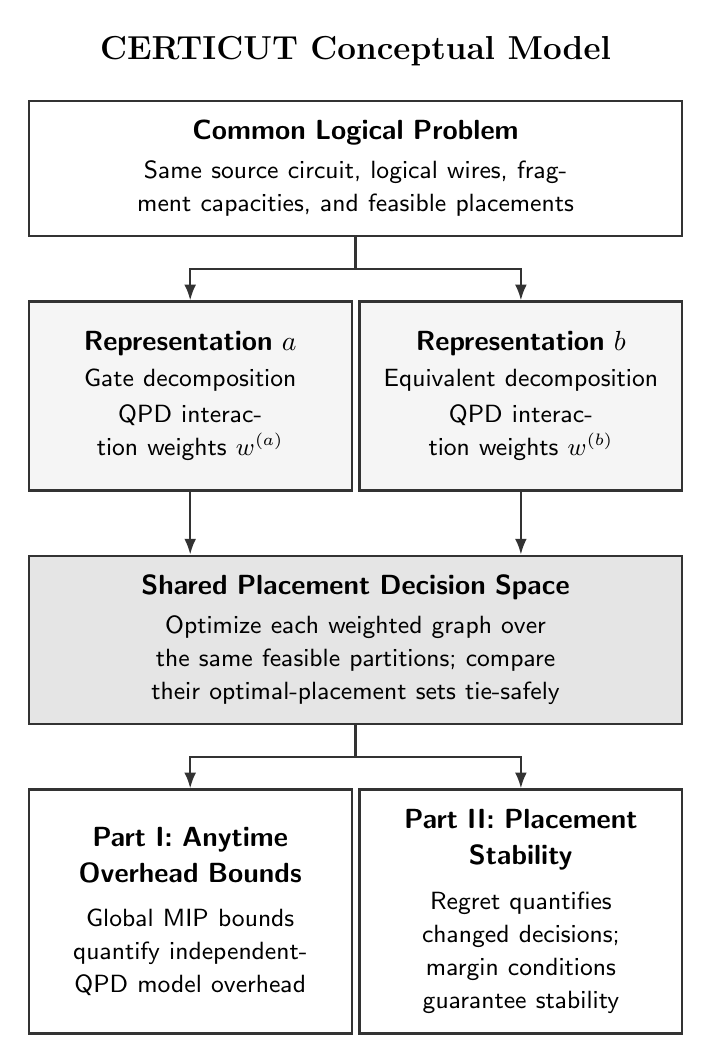
\begin{tikzpicture}[
  font=\sffamily,
  >=Latex,
  arrow/.style={-{Latex[length=2mm,width=1.5mm]}, draw=black!80, line width=0.8pt},
  topbox/.style={draw=black!80, fill=white, line width=0.8pt, align=center,
    text width=78mm, inner sep=2.5mm},
  repbox/.style={draw=black!80, fill=black!4, line width=0.8pt, align=center,
    text width=37mm, minimum height=24mm, inner sep=2mm},
  midbox/.style={draw=black!80, fill=black!10, line width=0.8pt, align=center,
    text width=78mm, inner sep=2.5mm},
  outbox/.style={draw=black!80, fill=white, line width=0.8pt, align=center,
    text width=37mm, minimum height=28mm, inner sep=2mm}
]

% Title
\node[font=\bfseries\large] (title) {CERTICUT Conceptual Model};

% 1. Top node: Common Logical Problem
\node[topbox, below=3mm of title] (logical) {
  \textbf{Common Logical Problem}\\[2pt]
  \small Same source circuit, logical wires, fragment capacities, and feasible placements
};

% 2. Middle tier: Representation A vs Representation B
\node[repbox, anchor=north west] (repA) at ([yshift=-8mm]logical.south west) {
  \textbf{Representation $a$}\\[2pt]
  \small Gate decomposition\\[1pt]
  \small QPD interaction weights $w^{(a)}$
};

\node[repbox, anchor=north east] (repB) at ([yshift=-8mm]logical.south east) {
  \textbf{Representation $b$}\\[2pt]
  \small Equivalent decomposition\\[1pt]
  \small QPD interaction weights $w^{(b)}$
};

% 3. Decision space node
\node[midbox, anchor=north] (decision) at ([yshift=-8mm]$(repA.south)!0.5!(repB.south)$) {
  \textbf{Shared Placement Decision Space}\\[2pt]
  \small Optimize each weighted graph over the same feasible partitions; compare their optimal-placement sets tie-safely
};

% 4. Part I vs Part II Outcomes (equal minimum height 30mm)
\node[outbox, anchor=north west, minimum height=31mm] (part1) at ([yshift=-8mm]decision.south west) {
  \textbf{Part I: Anytime}\\[1pt]
  \textbf{Overhead Bounds}\\[4pt]
  \small Global MIP bounds quantify independent-QPD model overhead
};

\node[outbox, anchor=north east, minimum height=31mm] (part2) at ([yshift=-8mm]decision.south east) {
  \textbf{Part II: Placement}\\[1pt]
  \textbf{Stability}\\[4pt]
  \small Regret quantifies changed decisions; margin conditions guarantee stability
};

% Arrows
\draw[arrow] (logical.south) -- ++(0,-4mm) -| (repA.north);
\draw[arrow] (logical.south) -- ++(0,-4mm) -| (repB.north);

\draw[arrow] (repA.south) -- (repA.south |- decision.north);
\draw[arrow] (repB.south) -- (repB.south |- decision.north);

\draw[arrow] (decision.south) -- ++(0,-4mm) -| (part1.north);
\draw[arrow] (decision.south) -- ++(0,-4mm) -| (part2.north);

\end{tikzpicture}
\end{document}
